

\tikzset{every picture/.style={line width=0.75pt}} %set default line width to 0.75pt        

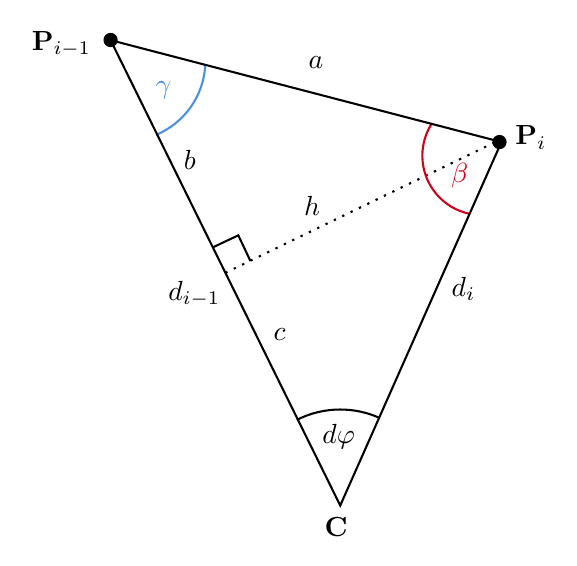
\begin{tikzpicture}[x=0.75pt,y=0.75pt,yscale=-1,xscale=1]
%uncomment if require: \path (0,269); %set diagram left start at 0, and has height of 269

%Straight Lines [id:da6739847496898159] 
\draw  [dash pattern={on 0.84pt off 2.51pt}]  (122.83,126.01) -- (252.88,63) ;
%Shape: Arc [id:dp4878212457791631] 
\draw  [draw opacity=0] (240.62,97.61) .. controls (227.55,94.98) and (217.71,83.44) .. (217.71,69.6) .. controls (217.71,63.88) and (219.39,58.55) .. (222.28,54.08) -- (246.29,69.6) -- cycle ; \draw  [color={rgb, 255:red, 208; green, 2; blue, 27 }  ,draw opacity=1 ] (240.62,97.61) .. controls (227.55,94.98) and (217.71,83.44) .. (217.71,69.6) .. controls (217.71,63.88) and (219.39,58.55) .. (222.28,54.08) ;
%Shape: Arc [id:dp901574933751006] 
\draw  [draw opacity=0] (113.13,25.58) .. controls (112.48,40.91) and (102.88,53.93) .. (89.43,59.54) -- (74.58,23.92) -- cycle ; \draw  [color={rgb, 255:red, 74; green, 144; blue, 226 }  ,draw opacity=1 ] (113.13,25.58) .. controls (112.48,40.91) and (102.88,53.93) .. (89.43,59.54) ;
%Shape: Polygon [id:ds6190617836836185] 
\draw   (67.51,13.91) -- (255.81,63) -- (178.15,238.12) -- cycle ;
%Shape: Ellipse [id:dp4849771561113211] 
\draw  [fill={rgb, 255:red, 0; green, 0; blue, 0 }  ,fill opacity=1 ] (251.95,63) .. controls (251.95,61.38) and (253.26,60.07) .. (254.88,60.07) .. controls (256.5,60.07) and (257.81,61.38) .. (257.81,63) .. controls (257.81,64.62) and (256.5,65.93) .. (254.88,65.93) .. controls (253.26,65.93) and (251.95,64.62) .. (251.95,63) -- cycle ;
%Shape: Circle [id:dp8356396848663105] 
\draw  [fill={rgb, 255:red, 0; green, 0; blue, 0 }  ,fill opacity=1 ] (64.58,13.84) .. controls (64.58,12.22) and (65.89,10.91) .. (67.51,10.91) .. controls (69.13,10.91) and (70.44,12.22) .. (70.44,13.84) .. controls (70.44,15.46) and (69.13,16.77) .. (67.51,16.77) .. controls (65.89,16.77) and (64.58,15.46) .. (64.58,13.84) -- cycle ;
%Shape: Arc [id:dp8012007227541399] 
\draw  [draw opacity=0] (157.23,196.86) .. controls (163.51,193.67) and (170.62,191.87) .. (178.15,191.87) .. controls (184.79,191.87) and (191.12,193.27) .. (196.83,195.8) -- (178.15,238.12) -- cycle ; \draw   (157.23,196.86) .. controls (163.51,193.67) and (170.62,191.87) .. (178.15,191.87) .. controls (184.79,191.87) and (191.12,193.27) .. (196.83,195.8) ;
%Shape: Right Angle [id:dp07010543377164635] 
\draw   (116.98,113.65) -- (129.04,107.95) -- (134.88,120.31) ;

% Text Node
\draw (161.42,20.19) node [anchor=north west][inner sep=0.75pt]   [align=left] {$\displaystyle a$};
% Text Node
\draw (159.22,87.59) node [anchor=north west][inner sep=0.75pt]   [align=left] {$\displaystyle h$};
% Text Node
\draw (230.37,126.44) node [anchor=north west][inner sep=0.75pt]   [align=left] {$\displaystyle d_{i}$};
% Text Node
\draw (93.81,128.37) node [anchor=north west][inner sep=0.75pt]   [align=left] {$\displaystyle d_{i-1}$};
% Text Node
\draw (168.08,197.65) node [anchor=north west][inner sep=0.75pt]   [align=left] {$\displaystyle d\varphi $};
% Text Node
\draw (230.1,71.96) node [anchor=north west][inner sep=0.75pt]  [color={rgb, 255:red, 208; green, 2; blue, 27 }  ,opacity=1 ] [align=left] {$\displaystyle \beta $};
% Text Node
\draw (87.69,32.2) node [anchor=north west][inner sep=0.75pt]  [color={rgb, 255:red, 74; green, 144; blue, 226 }  ,opacity=1 ] [align=left] {$\displaystyle \gamma $};
% Text Node
\draw (101.34,65.61) node [anchor=north west][inner sep=0.75pt]   [align=left] {$\displaystyle b$};
% Text Node
\draw (144.57,151.34) node [anchor=north west][inner sep=0.75pt]   [align=left] {$\displaystyle c$};
% Text Node
\draw (169.08,242.2) node [anchor=north west][inner sep=0.75pt]   [align=left] {$\displaystyle \mathbf{C}$};
% Text Node
\draw (261,53.76) node [anchor=north west][inner sep=0.75pt]   [align=left] {$\displaystyle \mathbf{P}_{i}$};
% Text Node
\draw (28.06,8.4) node [anchor=north west][inner sep=0.75pt]   [align=left] {$\displaystyle \mathbf{P}_{i-1}$};


\end{tikzpicture}

